%
% fig-volint.tex
%
% (c) 2025 Prof Dr Andreas Müller
%
\begin{figure}
\centering
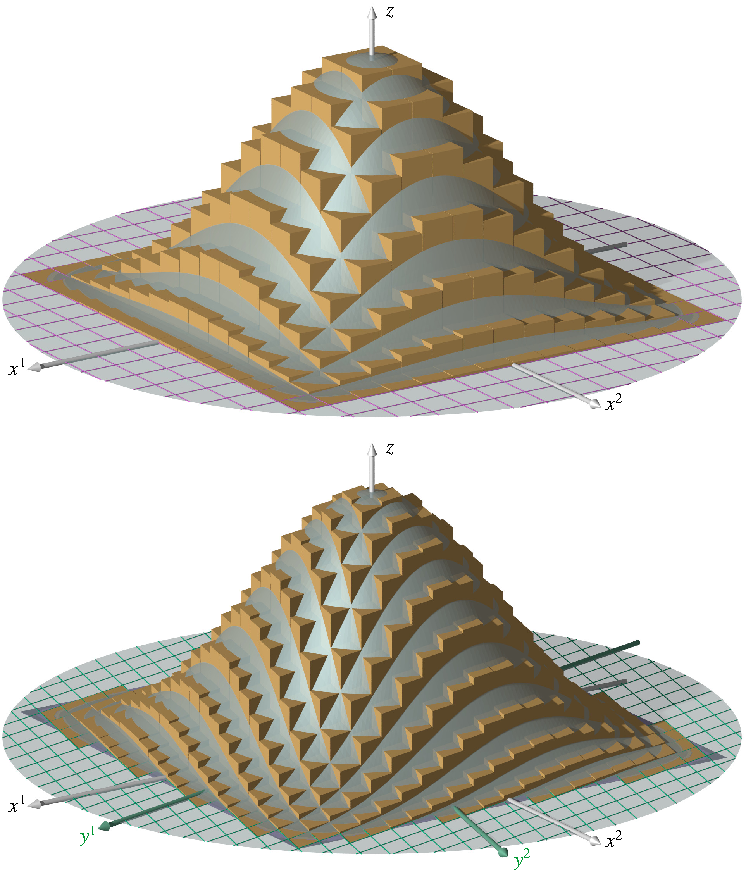
\includegraphics[width=\textwidth]{chapters/040-green/images/volint.pdf}
\caption{Volumen unter dem Graphen der Funktion $f(x^1,x^2)$ berechnet mit
zwei verschiedenen Parametrisierungen der Ebene.
In den $(x^1,x^2)$-Koordinaten wird das Volumen als Summe von Quadern
approximiert.
In den $(y^1,y^2)$-Koordinaten werden Prismen mit parallelogrammförmigen
Grundflächen aufaddiert.
Eine koordinatenunabhängige Grösse entsteht nur, wenn die Änderung
der Prismengrundfläche berücksichtigt wird.
\label{buch:green:fig:volint}}
\end{figure}
